\begin{figure}
	\centering
	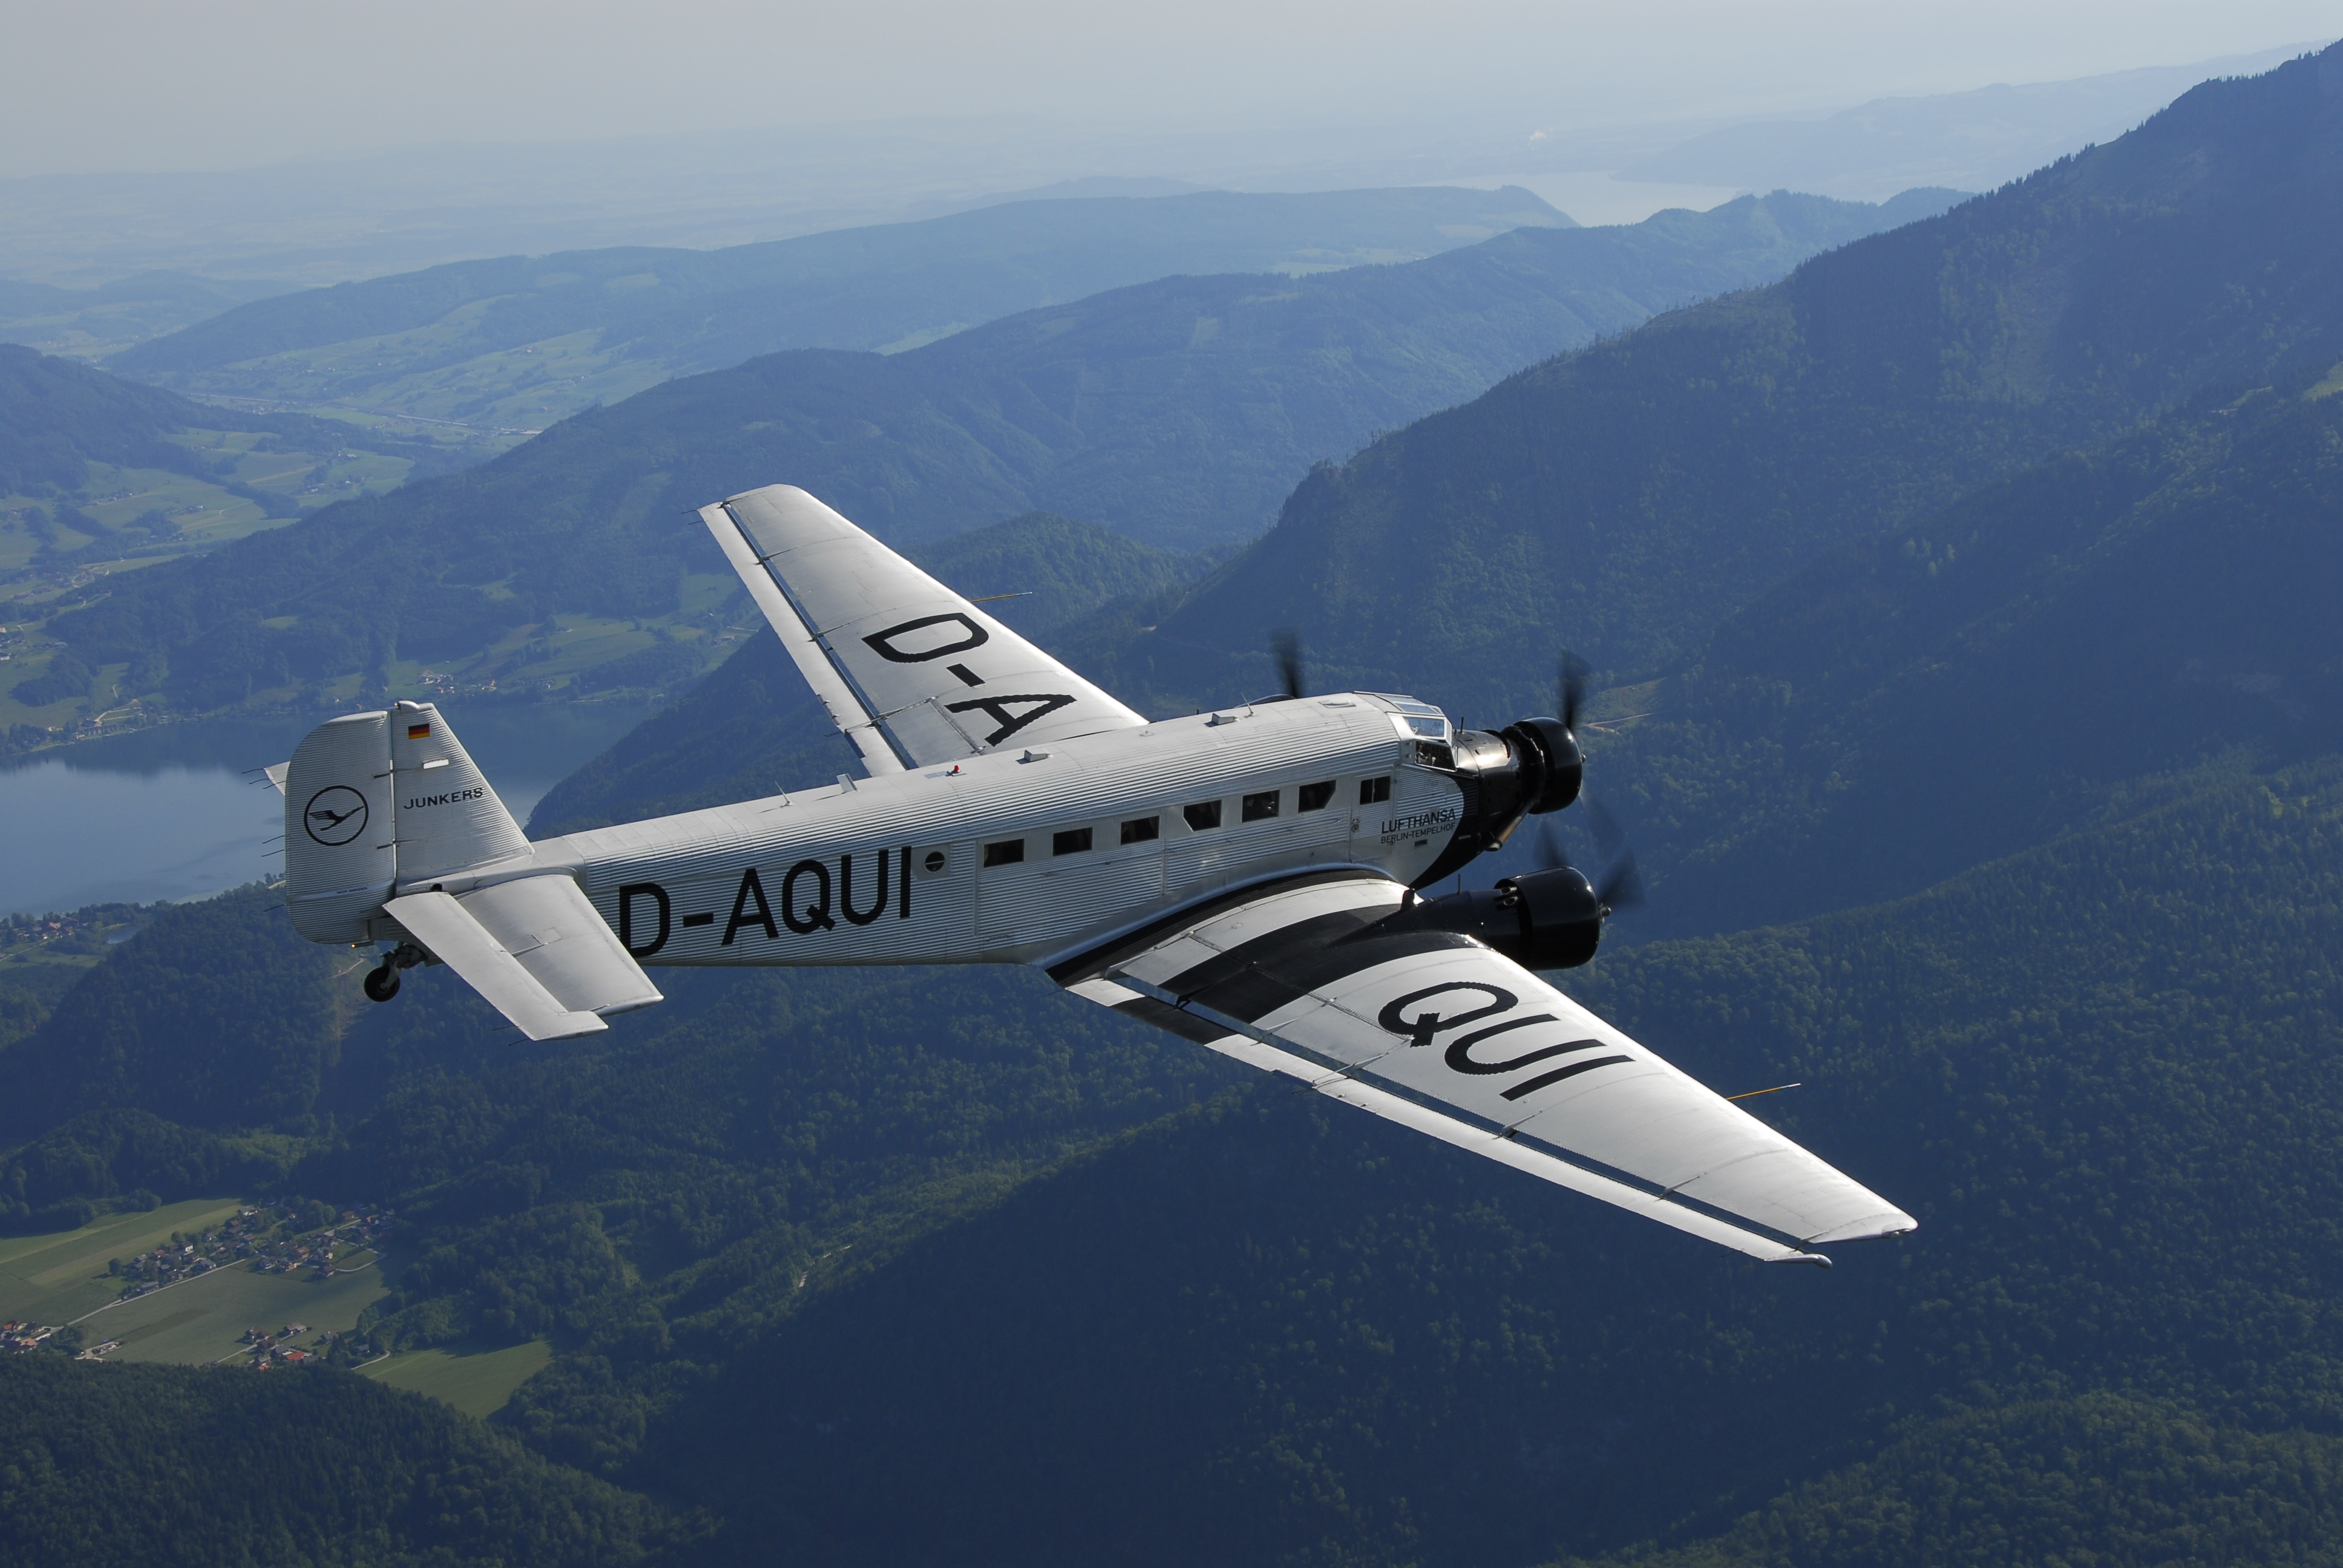
\includegraphics[width=0.65\textwidth]{papers/joukowski/images/04_komplexe_analysis/Ju_52.jpg}
	\caption{
		Die Ju-52 hat hinter dem Hauptflügel einen kleinen Hilfsflügel, der den Auftrieb nochmals vergrössert. Das Flügelprofil besteht somit aus zwei getrennten Teilen und kann somit nicht mit unserem Modell beschrieben werden. 
	}
\end{figure}
